\section{Proposed Solution}

Building on the identified limitations of traditional input devices, which contribute to ergonomic strain and accessibility barriers, this chapter introduces a wearable air mouse glove. This solution is engineered to provide an intuitive, natural, and inclusive human-computer interaction mechanism by tracking three-dimensional hand movements and tactile feedback.

\subsection{System Concept and Interaction Mechanisms}

The proposed solution is an integrated wearable air mouse, designed as a lightweight, ergonomic glove that translates natural hand gestures into precise digital interface controls. This system represented in Figure \ref{fig:sketch} moves beyond the limitations of traditional desktop mice by utilizing a combination of inertial sensing, conductive textile interfaces, and wireless communication protocols. At its core, the device functions as a Human Interface Device (HID) that maps three-dimensional spatial movements to two-dimensional cursor coordinates, while providing discrete finger-based triggers for standard mouse operations such as clicking and scrolling. By embedding the control interface directly onto the user's hand, the solution offers a more intuitive and mobile interaction model suitable for presentations, virtual reality environments, and ergonomic computing.

\begin{figure}[h]
    \centering
    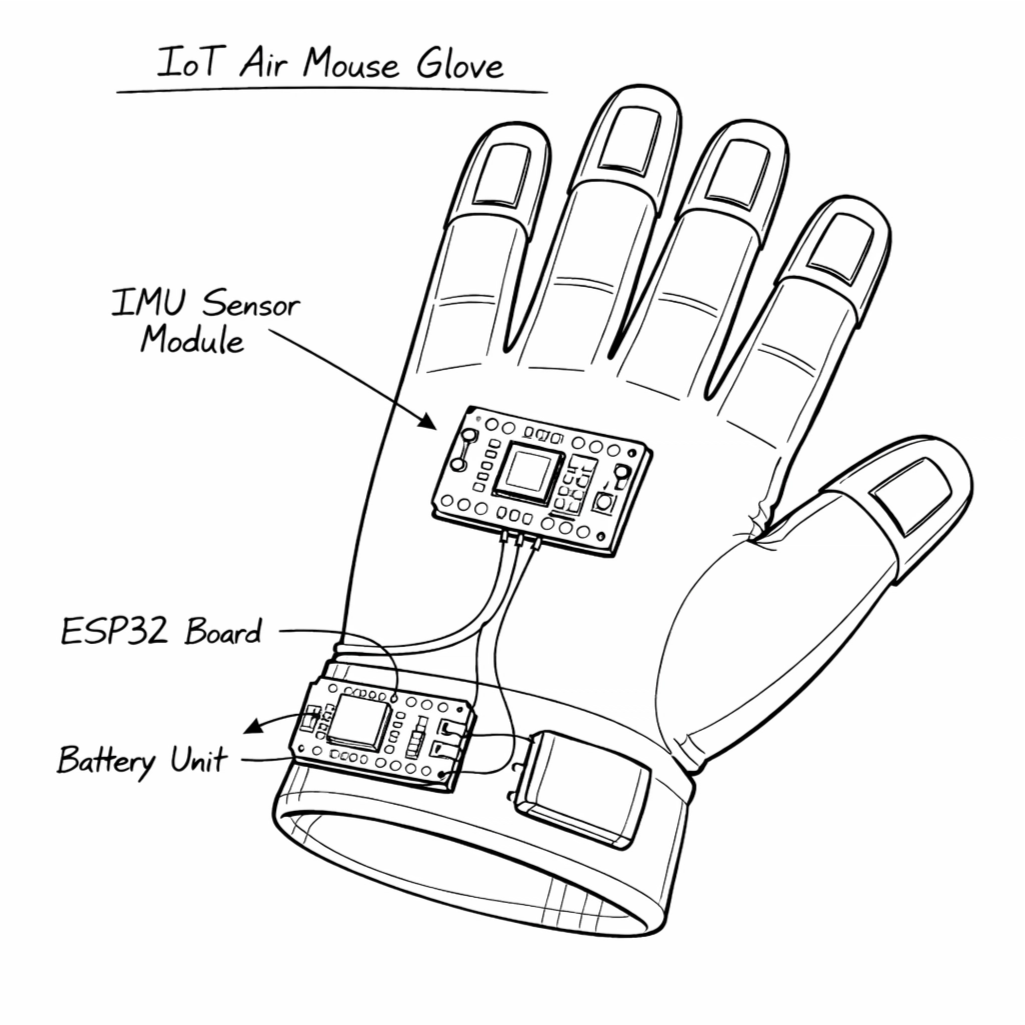
\includegraphics[width=0.5\textwidth]{img/air_mouse_glove_sketch.png}
    \caption{Conceptual Sketch of the AirGlove}
    \label{fig:sketch}
    
\end{figure}

The primary mechanism for motion tracking is centered around a high-precision Inertial Measurement Unit (IMU), such as the MPU6050 or MPU6500. These sensors integrate a three-axis accelerometer and a three-axis gyroscope to capture both linear acceleration and angular velocity. Through the use of onboard Digital Motion Processing (DMP) and sensor fusion algorithms the system can accurately determine the orientation and tilt of the hand while filtering out mechanical noise and drift. This data is then translated into cursor movement, where the gyroscope handles fine rotational adjustments and the accelerometer detects broader directional shifts. For simpler implementations or power-constrained scenarios, a standalone three-axis accelerometer like the ADXL345 can be employed to detect basic tilt-based movement, though the 6-axis IMU remains the standard for professional-grade responsiveness \cite{mummadi2018imu_glove}.


To facilitate user interaction, the glove incorporates strategically placed finger contact points and conductive pathways. These contact points, typically located on the tips of the index and middle fingers and the side of the thumb, utilize conductive fabrics or silver-plated threads to act as soft, wearable switches. When the user brings the thumb into contact with a specific finger pad, a circuit is closed, which the system interprets as a left-click, right-click, or scroll activation. This textile-based approach ensures that the glove remains flexible and comfortable for extended use, avoiding the bulk of traditional mechanical buttons. Furthermore, the integration of a dedicated sensitivity switch allows users to dynamically adjust the control gain. This hardware-level toggle enables the microcontroller to scale the sensor data in real-time, allowing the user to switch between high-sensitivity modes for rapid navigation and low-sensitivity modes for precision tasks like digital drawing or detailed selection.

The processing and communication hub of the device is the ESP32 microcontroller, chosen for its powerful dual-core architecture and integrated wireless capabilities. The ESP32 handles the real-time acquisition of sensor data via I2C or SPI interfaces, executes the gesture recognition logic, and manages the Bluetooth Low Energy (BLE) or 2.4GHz HID profile to communicate with the host computer. This allows the glove to appear as a standard wireless mouse to any operating system without requiring specialized drivers \cite{prayogi2024esp32_airmouse}.

% \begin{figure}[h]
%     \centering
%     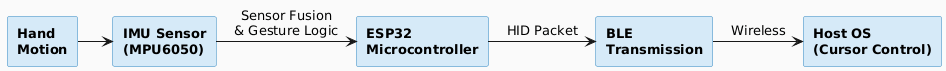
\includegraphics[width=1\textwidth]{img/flow.png}
%     \caption{Processing Flow}
%     \label{fig:processing_flow}
    
% \end{figure}

% At the system level, the glove's operation can be described as a closed sensing processing communication pipeline, illustrated in Figure \ref{fig:processing_flow}. Motion data is continuously sampled by the IMU at a configurable rate, transmitted to the ESP32, where a firmware layer applies sensor fusion and gesture classification. Valid gesture events — such as a sustained tilt beyond a defined angular threshold or a finger contact closure — are encoded into standard HID mouse report packets and transmitted via BLE to the paired host device. The host operating system processes these packets identically to any USB or Bluetooth mouse, requiring no custom drivers. This architecture ensures low latency between physical gesture and cursor response, while the modular firmware structure allows future extension to support additional gestures such as scroll, zoom, or multi-finger shortcuts.
